% !TEX root = ../preamble.tex

\section{Implementation}

\subsection{String alignment}
This section describes how roles are being aligned in the dataset in order to get more accurate results.\\
The data containing the roles and the string describing the actual role contains superfluous information, e.g. the id of the actor, the id of the movie. The string describing the role can for instance contain information defining what specific policeman it was. In order to generalise the roles such information is removed, e.g. there is no difference between policeman \#1 and policeman \#2 in the cleaned dataset. Additionally unspecified roles are deleted. As an example multiple people has had a role playing themselves. Such a role is defined as “Themselves” in the dataset, which is very general and not an actual role, hence these are deleted. Other similar roles, e.g. "himself", "herself", "extra" or "additional" are removed as well. Some roles define which year the role was from. This information is also removed. Finally, many of the string describing the roles are empty. These entries are deleted.

\subsection{Data processing}
There are multiple ways to handle the data that needs to be processed.
One approach is to load all the data into the RAM. This technique is very demanding on the RAM, since everything is stored. Storing everything in the RAM has some clear advantages e.g. being able to go back and forth in the data or reading the same subset of the data multiple times. However if the size of the data exceeds the amount of RAM available, one might experience severe performance implications, due to e.g. memory swapping.
Some datasets have a size which makes it impractical, sometimes even impossible, to store them in the RAM. This constraint leads to another approach, which is to stream the data. Streaming the data has advantages as well as disadvantages. Only a fraction of the whole data is stored in the RAM, imposing no extraordinary demand to the size of the available RAM. Only storing part of the data makes it cumbersome, and to some extent impossible, to go back and forth in the data.

\subsubsection{Movie wrangling}
The data obtained from imdb has been filtered to fit the problem. The movie data considered when comparing movies are the following:
\begin{itemize}
\item Title
\item Director ids
\item Actor ids
\item Genres as strings
\end{itemize}
The movies are loaded in RAM and the attributes are stored in sets. The sets that is used as an input to jaccard similarity coefficient calculation is the union of all the sets. Movies with less than \(x\) elements in the union set is not used as input for similarity sensitive hashing.

\subsection{Practical space consumption}
The following logarithmic graph is the number of map entries used by Misra Gries, reservoir sampling and the naive solution based on the concrete data set. The vertical axis is space consumption and the horizontal axis is \(\alpha\). Only the naïve solution is dependent on the size of the concrete example and not on \(\alpha\). The reservoir sampling algorithm is linear dependent on the threshold.
\begin{figure}[H]
	\centering
	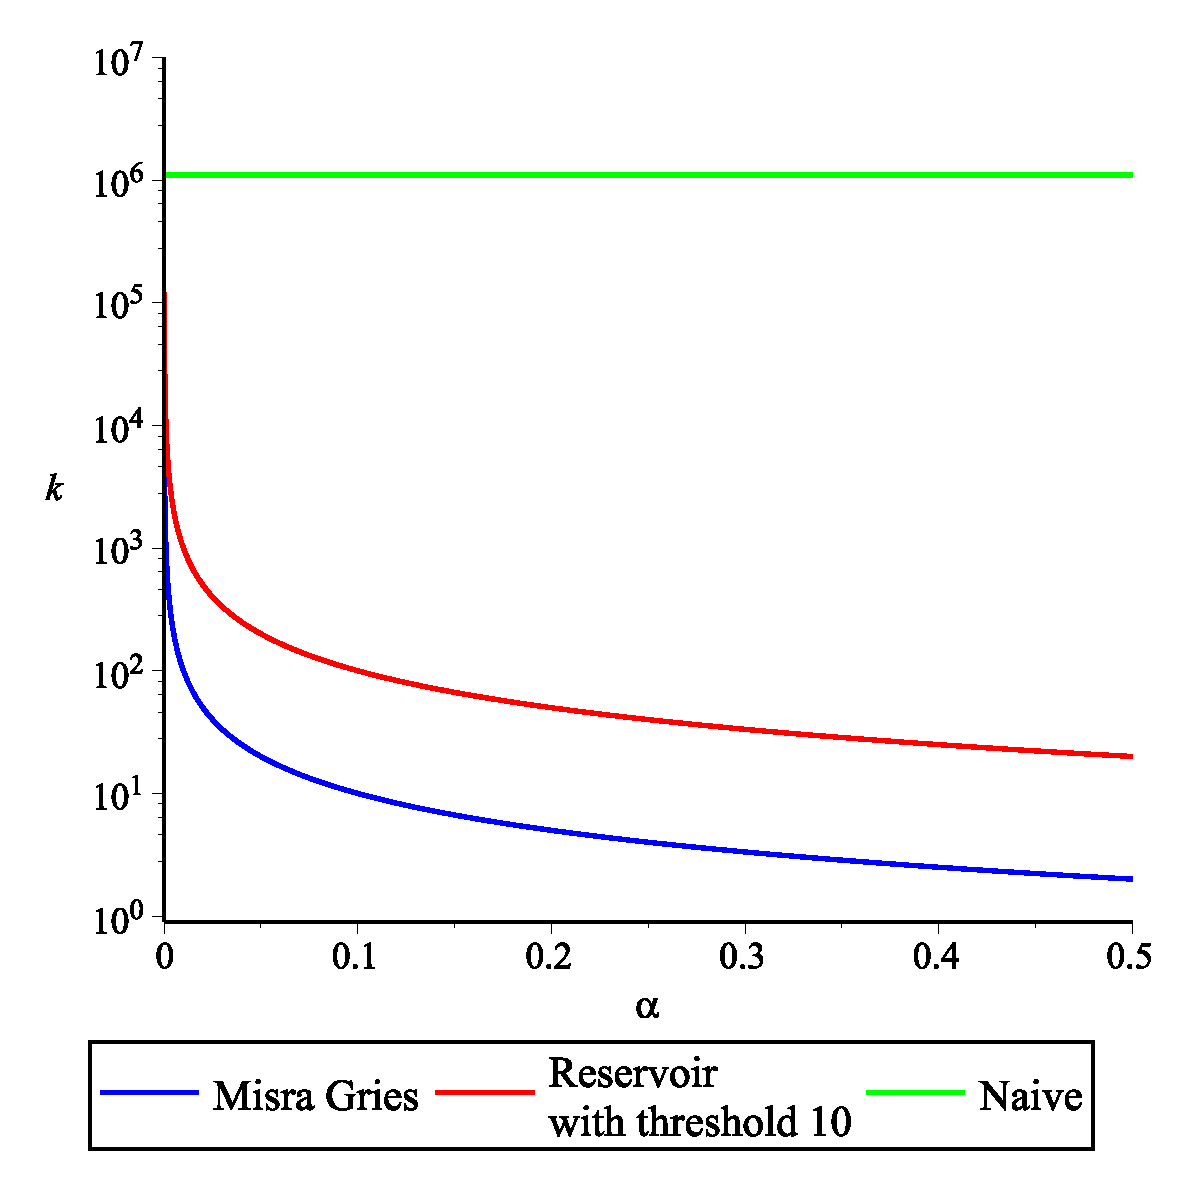
\includegraphics[width=290px]{img/streamingMemoryGraph.eps}
	\caption{Space consumption}
	\label{fig:space_consumption}
\end{figure}
As seen in figure~\ref{fig:space_consumption} the space used by the naïve solution is 1000 times as large as the space used by Misra Gries and reservoir sampling. when looking for elements in Hwith =0.001. The size of the data stream is approximately 2.3 million.
\\ \\ \\ \\
\subsection{Applications}
Locality-sensitive hashing have a wide range of applications where it proves to be relevant and quite popular. Here is mentioned a small part of the applications.  \\
It is specifically widely used in the field of "Nearest neighbor search"; data compression, databases, data mining, image- and video-databases, machine learning, pattern recognition, etc. all use locality-sensitive hashing and especially when the dimensions of the problem are high, is the algorithm efficient. 
It is also used in combination with the "k-nearest neighbors algorithm", also known as "k-nn", which is widely used, among others, in the fields of machine learning and recommender systems such as those used by Netflix\footnote{\url{www.netflix.com}} and Pandora\footnote{\url{www.pandora.com}}. Applications doing video- and Audio-fingerprinting, such as Shazam\footnote{\url{www.shazam.com}} and Youtube\footnote{\url{www.youtube.com}} can also use the algorithm in order to find music tracks that sounds most alike, as done by Shazam, or to automatically remove videos containing illegal footage, as done by Youtube.

\subsection{Shingling}
The purpose of the shingling step is, for each input point, to create n-grams, with size \(w\), of tokens from that input point. Tokens are the attributes one wants to base the comparison of the inputs points on; e.g. for document comparison, this could be words and for comparing movies it might be genres. All shinglings are later used to create a signature for that input point on order for it to be compared with others at a later point. 
\subsubsection{Choosing the length, \(w\), of shingles}
The length of shingles impact both the space consumption and the running time of the algorithm. The lower the number, the higher possible amount of unique shingles. Also, with a \(w\) value above 1, the order of the tokens become relevant, which is important in a number of cases, e.g. when comparing documents. If \(w\) is 1, then all words in all documents are theoretically compared, and a lot of documents will have a lot in common, with basic words like "the" and "and", however with a \(w\) value of e.g. 10, only documents with 10 words in the same order will be considered as similar, thus giving more relevant/true results. In the case of comparing movies, order is completely irrelevant and all tokens should be compared to each other. This means that w=1 is the only relevant value for this problem.